% There are two copyright options: copyright and copyright. Seriously,
% the choice boils down to whether you're going to file copyright through
% ProQuest. If you will, use the copyright option.
\documentclass[dissertation,notoc,openany]{tufte-book}
%\documentclass[dissertation,copyright,notoc,openany]{tufte-book}

\setcounter{secnumdepth}{0}
%\setcounter{chapter}{5}

\bibliographystyle{uabibnat}

%%
% To use accents
\usepackage[utf8]{inputenc}

%%
% For nicely typeset tabular material
\usepackage{booktabs}

%%
% For graphics / images
\usepackage{graphicx}
\setkeys{Gin}{width=\linewidth,totalheight=\textheight,keepaspectratio}
\graphicspath{{figs/}}

\usepackage[export]{adjustbox}

% The fancyvrb package lets us customize the formatting of verbatim
% environments.  We use a slightly smaller font.
\usepackage{fancyvrb}
\fvset{fontsize=\normalsize}

%%
% Prints a trailing space in a smart way.
\usepackage{xspace}

%%
% specifying and applying colors
\usepackage{color}

%%
% For table color backgrounds
\usepackage{colortbl}

%%
% for code listings (e.g., R)
\usepackage{listings}

%% color definitions
\definecolor{lightgray}{rgb}{0.96, 0.955, 0.945}
\definecolor{numbergray}{rgb}{0.7, 0.7, 0.7}
\definecolor{midgray}{rgb}{0.5, 0.5, 0.5}
\definecolor{deepred}{rgb}{0.9,0.1,0.1}
\definecolor{lightred}{rgb}{0.975, 0.925, 0.925}

% listing add'l keywords
\lstset{emph={%  
    auc
    },emphstyle={\color{red}}%
}%

\lstdefinestyle{rstyle}{
	language=R,
    backgroundcolor=\color{lightgray},
    commentstyle=\color{midgray},
    keywordstyle=\color{red},
    basicstyle=\scriptsize\ttfamily,
    breakatwhitespace=true,
    breaklines=true,
    keepspaces=true,
    framextopmargin=0pt,
    showspaces=false,
    showstringspaces=false,
    showtabs=false,
    stringstyle=\ttfamily,
    tabsize=2
}
 
\lstset{style=rstyle}

%%
% Sometimes you want a full-page figure with no margin notes.
\newenvironment{pagefigure}{%
	\begin{figure*}[p]
	\classiccaptionstyle
}{\end{figure*}}

%%
% Sometimes you want a full-page table with no margin notes.
\newenvironment{pagetable}{%
	\begin{table*}[p]
	\classiccaptionstyle
}{\end{table*}}

%%
% Would otherwise be `Bibliography', but UA requires `References'
\renewcommand{\bibname}{References}

%%
% Prints argument within hanging parentheses (i.e., parentheses that take
% up no horizontal space).  Useful in tabular environments.
\newcommand{\hangp}[1]{\makebox[0pt][r]{(}#1\makebox[0pt][l]{)}}

%%
% Prints an asterisk that takes up no horizontal space.
% Useful in tabular environments.
\newcommand{\hangstar}{\makebox[0pt][l]{*}}

%%
% Emphasize table result
\newcommand{\redem}[1]{\textcolor{deepred}{\textbf{#1}}}

%%
% mark TODOs
\newcommand{\todo}[1]{\textcolor{red}{TODO: #1}}

%%
% mark edits
\newcommand{\edit}[1]{\textcolor{blue}{#1}}

%%
% Improve chapter title appearance
\makeatletter
\titleformat{\chapter}%
  [block]% shape
  {\relax\ifthenelse{\NOT\boolean{@tufte@symmetric}}{\begin{fullwidth}}{}}% format applied to label+text
  {\itshape\huge\thechapter\quad}% label
  {0pt}% horizontal separation between label and title body
  {\huge\rmfamily\itshape}% before the title body
  [\ifthenelse{\NOT\boolean{@tufte@symmetric}}{\end{fullwidth}}{}]% after the title body
\makeatother

%%
% More space between figure numbers and titles
\makeatletter
     \renewcommand*\l@figure{\@dottedtocline{1}{1em}{2.2em}}
\makeatother

%%
% more space between table numbers and titles
\makeatletter
     \renewcommand*\l@table{\@dottedtocline{1}{1em}{2em}}
\makeatother

%%
% Repeated values, esp in front material.
\completetitle{A Clever Pun: An Explanatory Subtitle}
\fullname{Raymond Quentin Smuckles} % Full name (including middle etc.)
\degreename{Doctor of Philosophy}	% Title of your degree.
\title{A Clever Pun: An Explanatory Subtitle}
\author{Raymond Quentin Smuckles}

% Generates the index, if you create one. (Does nothing, otherwise.)
\usepackage{makeidx}
\makeindex

\begin{document}

\begin{fullwidth}
% Set up the title page
\maketitlepage
{DEPARTMENT OF NEUROASTROLOGY}	% Title of your department.
{3030}

% Insert the approval form.  Note that for electronic submission
% of your Ph. D. dissertation, you must bring *two* copies of the
% approval page to your final defense.  These must be signed by
% the committee. 
\approval
{February 30, 3030}		% Defense Date	
{Cassandra Kazenzakis}		% Dissertation Director
{Cassandra Kazenzakis}		% 1st committee member
{Cornelius Bear}		% 2nd committee member
{Lyle Roscoe Gabriel}	% 3rd committee member
%{} % 4th committee member (leave empty if None)
%{} % 5th committee member (leave empty if None)

% Include the ``Statement by Author'' for Dissertations
\statementbyauthor
\statementbyauthor % Yes, you need the second one of these.
% If this is a Thesis, use the following form, with your thesis director's
% name and title in the square brackets like so (you should also omit the 
% approval form insertion above):
%\statementbyauthor[Jane M. Doe\\Professor of Chemistry]

% Include the ``Acknowledgements''
% NB: Strongly encouraged
\incacknowledgements{acknowledgements}

% Include the ``Dedication''
% NB: optional
\incdedication{dedication}

% Create a ``Table of Contents''
% NB: required
\tableofcontents

% Create a ``List of Figures''
% NB: Strongly encouraged
\listoffigures

% Create a ``List of Tables''
% NB: Strongly encouraged
\listoftables

% Include the ``Abstract''
% NB: required
\incabstract{abstract}

\end{fullwidth}

% Include the various chapters
\chapter{Introduction}
\label{chapter:introduction}

\newthought{The introduction chapter} begins here, starting with small caps like Tufte does, using the \verb|\newthought| command (which you can also use to start a new thought within a section. This style is based on Edward Tufte's (TOUGH-tee) books.\cite{Tufte2001,Tufte1990,Tufte1997,Tufte2006} There are many cheats and shortcuts to approximate Tufte's style, like using Palatino, Helvetica, and Bera Mono rather than Tufte's actual fonts like Bembo and Gill Sans. More detail about what styles to use within this class, see \href{https://ctan.org/pkg/tufte-latex}{Tufte Latex}.

\section{Floats}\label{sec:overview}

\newthought{Each section} also starts with small caps. Okay, you probably noticed the huge margins. You don't necessarily have to use them all the time. For example, I could cite Tufte here~\citep{Tufte2001} by using the \verb|\citep| instead of the \verb|\cite| command, which makes marginal citations.

\subsection{Subsection}

By the way, there are subsections, but no sub-subsections. This is on purpose.

\begin{marginfigure}%
  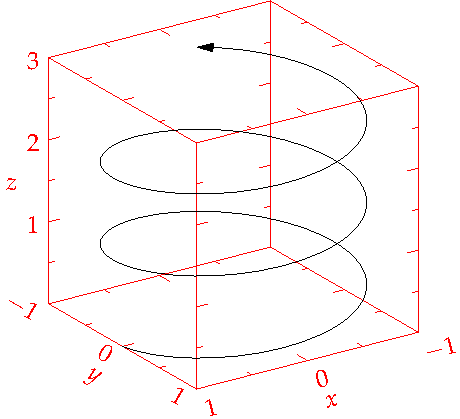
\includegraphics[width=\linewidth]{introduction/helix}
  \caption{This is a margin figure.  The helix is defined by 
    $x = \cos(2\pi z)$, $y = \sin(2\pi z)$, and $z = [0, 2.7]$.  The figure was
    drawn using Asymptote (\url{http://asymptote.sf.net/}).}
  \label{fig:marginfig}
\end{marginfigure}

\paragraph{Paragraph} 

The paragraph command is as small as it gets.

\subsection{Floats again}

Anyway, part of the reason to use this class is the use of sidenotes\sidenote{Like this one, introduced with \texttt{sidenote} or \texttt{footnote}.} and margin notes. Margin notes work the same but have no superscript to refer back to the text.

You can also put figures and tables in the margins using the \texttt{marginfigure} and \texttt{margintable} environments, and reference them as normal, like Fig.~\ref{fig:marginfig}. A trick with these is that they sometimes run into each other, in which case you should use the optional offset like \verb|\begin{margintable}[-5em]|. Similar options exist for sidenotes and margin notes, so checkout \href{https://ctan.org/pkg/tufte-latex}{Tufte LaTeX} for more info. Sidenotes are also great for short code listings.\footnote{\vspace{-1em}\begin{lstlisting}^^J
glm(y ~ m * x + b, 
    family = "binomial")^^J
\end{lstlisting}
}

Anyway, of course not everything can go in the margin, and for that we have the \texttt{figure} and \texttt{figure*} environment, for normal text width and full page width, respectively.
\begin{figure*}[h]
  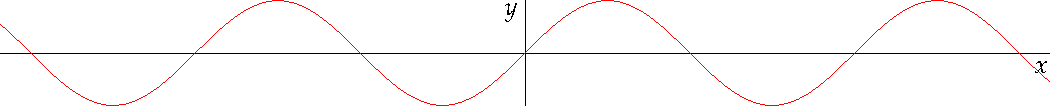
\includegraphics[width=\linewidth]{introduction/sine.pdf}%
  \caption{This graph shows $y = \sin x$ from about $x = [-10, 10]$.
  \emph{Notice that this figure takes up the full page width.}}%
  \label{fig:fullfig}%
\end{figure*}

\begin{figure}
  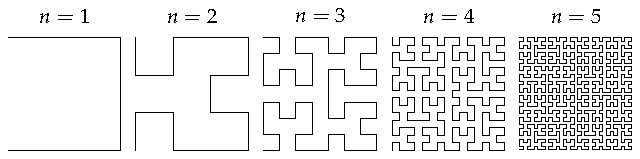
\includegraphics{introduction/hilbertcurves.pdf}
%  \checkparity This is an \pageparity\ page.%
  \caption[Hilbert curves of various degrees $n$.][6pt]{Hilbert curves of various degrees $n$. \emph{Notice that this figure only takes up the main textblock width.}}
  \label{fig:textfig}
  %\zsavepos{pos:textfig}
\end{figure}

\section{By the way}

Please use \texttt{booktabs}-style tables, please. Please. They look like Table~\ref{tab:example}.

\begin{table}[h]
\centering
\begin{tabular}{l l l l}
\toprule
\textit{Name}	& \textit{Species}	& \textit{Age}	& \textit{Smell}	\\
\midrule
Phillipe		& Otter				& 5			& musky					\\ \rowcolor{lightgray}
T\'{e}odor		& Bear				& $\sim$35	& bachelor-esque		\\
Molly			& Cat				& $>$100	& fresh laundry			\\ \rowcolor{lightgray}
Liebot			& Robot				& ???		& Drakkar Noir			\\
\bottomrule
\end{tabular}
\caption{The way that tables should look.}
\label{tab:example}
\end{table}

\vspace{1em}
The zebra-striping (achieved using \verb|\rowcolor|) and title italics are optional, but the point is not to have a thousand thick black lines obscuring the information. Analogous to figures, variants \texttt{margintable}, \texttt{table}, and \texttt{table*} exist. Please just don't use them to make tables like \ref{tab:ugly}.
\begin{margintable}
\centering
\begin{tabular}{|l|l|l|}
\hline
\textbf{Alg}	& \textbf{P}		& \textbf{AUC}		\\ \hline\hline
BF-1000	& \textbf{$\mathbf{0.67}$**}	& \textbf{$\mathbf{0.81}$**}	\\ \hline
MTG-MN	& $0.54$			& $0.32$			\\ \hline
RM-DL2	& $0.33$			& $0.48$			\\ \hline
3CPO	& $0.45$			& $0.22$			\\ \hline
\end{tabular}
\caption{A distractingly ugly and overwrought margin table with obscure abbreviations.}
\label{tab:ugly}
\end{margintable}

\section{Speaking of which}

If you want it all to go together nicely, I suggest making figures in R. My favorite practical guide to making Tufte-like graphs is \href{http://motioninsocial.com/tufte/}{Tufte in R} by Lukasz Piwek.
%\include{chapters/review}
%\include{chapters/conclusion}

% Include the various appendices
\appendix
\chapter{An Example of an Appendix}\label{apndxA}

\begin{fullwidth}
You may choose to use the \texttt{fullwidth} environment to get rid of the margin if your appendix is just a list of words or something, e.g.: \begin{verbatim}
\begin{fullwidth}
Hello
\end{fullwidth}
\end{verbatim}
\end{fullwidth}

\backmatter

\begin{fullwidth}
%%
% Unfortunately, you have to manually set the page number before the 
% references start. This is because the Grad College insists their be no
% blank pages, and I haven't figured out how to do this besides manually
% setting the page count lower and then removing the blank page separately.
% I use pdftk for this, e.g.,
% pdftk A=dissertation.pdf B=watermarked_signatures.pdf cat A1 B1 3-91 93-end output dissertation_signed.pdf
% The above command takes the output of this file, substitutes a water-
% marked signature page for the second page, then cuts out page 92, and
% saves the result in dissertation_signed.pdf.
\setcounter{page}{91}
% Create the References list
\bibliography{dissertation}
\end{fullwidth}

\end{document}
